\documentclass[10pt,a4paper]{article}
\usepackage{amsmath}
\usepackage{amsfonts}
\usepackage{amssymb}
\usepackage{graphicx}
\usepackage[french]{babel}
\usepackage[T1]{fontenc}
\usepackage[utf8x]{inputenc}
\graphicspath{{images/}}
\usepackage{parskip}
\usepackage{fancyhdr}
\usepackage{vmargin}
\setmarginsrb{3 cm}{2.5 cm}{3 cm}{2.5 cm}{1 cm}{1.5 cm}{1 cm}{1.5 cm}

\title{Défis en Intelligence Artificielle}                             % Title
\author{Maxime De Wolf\\
		Dimitri Waelkens}                               % Author
\date{\today}                                           % Date

\makeatletter
\let\thetitle\@title
\let\theauthor\@author
\let\thedate\@date
\makeatother

\pagestyle{fancy}
\fancyhf{}
\rhead{\theauthor}
\lhead{\thetitle}
\cfoot{\thepage}

\begin{document}
   	
   	%%%%%%%%%%%%%%%%%%%%%%%%%%%%%%%%%%%%%%%%%%%%%%%%%%%%%%%%%%%%%%%%%%%%%%%%%%%%%%%%%%%%%%%%%
   	
   	\begin{titlepage}
   		\centering
   		\vspace*{0.5 cm}
   		
\includegraphics[scale = 0.75]{UMONS}\\[1.0 cm]   % University Logo
   		\textsc{\LARGE Université de Mons}\\[2.0 cm]   % University Name
   		\textsc{\large TP4}\\[0.5 cm]               % Course Name
   		\rule{\linewidth}{0.2 mm} \\[0.4 cm]
   		{ \huge \bfseries \thetitle}\\
   		\rule{\linewidth}{0.2 mm} \\[1.5 cm]
   		
   		\begin{minipage}{0.4\textwidth}
   			\begin{flushleft} \large
   				\emph{Auteur:}\\
   				\theauthor
   			\end{flushleft}
   		\end{minipage}~
   		\begin{minipage}{0.4\textwidth}
   			\begin{flushright} \large
   				\emph{Matricule: 151085}                                  % Your Student Number
   			\end{flushright}
   		\end{minipage}\\[2 cm]
   		
   		{\large \thedate}\\[2 cm]
   		
   		\vfill
   		
   	\end{titlepage}
   	
   	%%%%%%%%%%%%%%%%%%%%%%%%%%%%%%%%%%%%%%%%%%%%%%%%%%%%%%%%%%%%%%%%%%%%%%%%%%%%%%%%%%%%%%%%%
   	
   	\section{Configuration de \textit{Cartographer}}
   	
   		\begin{figure}[h]
   			\begin{center}
   				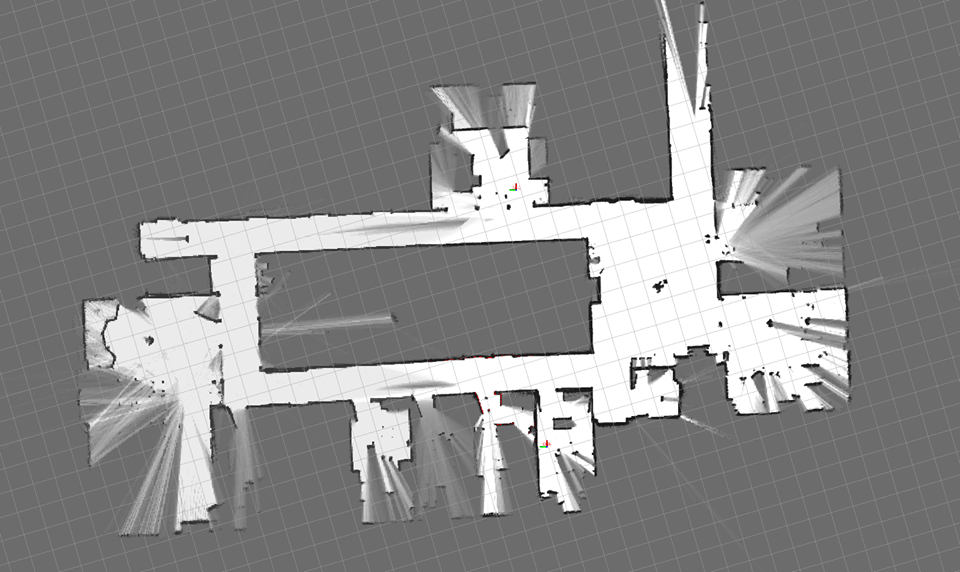
\includegraphics[width=0.75\linewidth]{map}
   			\end{center}
   			\caption{Carte obtenue grâce à \textit{Cartographer}}
   			\label{fig:map}
   		\end{figure}
   
   	\section{Localisation des objets}
   	
   		Cette section présente les résultats obtenus pour la détection d'objets que le robot à filmé. Nous expliquons donc dans un premier temps la logique que nous avons suivies pour obtenir ces résultats. Nous justifions ensuite la manière dont ils pourraient être améliorés.
   		
   		\subsection{Technique utilisée}
   		
   			Pour résoudre ce problème, nous utilisons une technique très simple. Effectivement, à chaque fois que le robot détecte un objet, nous repérons la position du robot ainsi que la distance à laquelle l'objet à été filmé. Cependant, nous avons également besoin de l'orientation du robot pour calculer la position de l'objet.
   			
   			Afin d'avoir l'orientation du robot, nous repérons également l'emplacement précédent duquel le robot voyait également cet objet. Nous pouvons donc calculer former par la droite passant par ces deux points dans le repère.
   			
   			Ensuite, grâce à la distance de l'objet filmé, nous pouvons déterminer la position de celui-ci.\\
   			
   			Le robot travaille sur un grand nombre d'image similaire. Nous calculons donc plusieurs fois la position du même objet.
   			
   			Pour pallier à ce problème nous utilisons un algorithme de \textit{clustering} simple afin de regrouper les position qui sont susceptible de représenter un même objet.
   			
   			Cette algorithme fonctionne de la manière suivante:
   			\begin{enumerate}
   				\item Pour chaque position, un regarde si elle est proche du centre d'un \textit{cluster} existant;
   				\item Si c'est le cas, on l'ajoute à ce \textit{cluster};
   				\item Sinon, on crée un nouveau \textit{cluster} qui contient cette position;
   			\end{enumerate}
   		
   			Finalement pour retrouver la position de chaque objet, on calcule le centre de chaque \textit{cluster}. Cette technique nous donne les résultats exposés par la Table \ref{tab:res}.
   	
   		\begin{table}[h]
   			\begin{center}
   				\begin{tabular}{|c|c|c|}
   					\hline
   					Objet & Position 1 & Position 2\\
   					\hline
   					\textit{teddy bear} & (2.399926850060335, -0.008283207609849293)& (12.604331235659147, 14.238862468344005) \\
   					\hline
   					\textit{motorbike} & (8.366541118657906, 14.943175542227172) & / \\
   					\hline
   					\textit{backpack}& (4.832979494372698, 2.7004257263585636) & / \\
   					\hline
   					\textit{suitcase} & (5.446312729568893, 16.221012094608028) & / \\
   					\hline
   					\textit{pottedplant} & (12.343678479509247, 14.322766597693517) & (0.9148871784197752, 23.25876369786711) \\
   					\hline
   					\textit{stop sign} & (7.87594829417553, 15.93296178462322) & / \\
   					\hline
   					\textit{refrigerator} & (6.239195085908132, 13.789541846887905) & / \\
   					\hline
   				\end{tabular}
   			\end{center}
   			\caption{Positions obtenues pour chaque objet détecté}
   			\label{tab:res}
   		\end{table}
   	
   		\subsection{Discussion sur les résultats}
   		
   		Grâce à la Table \ref{tab:res}, nous pouvons voir que nos résultats sont assez mauvais par rapport aux résultats attendus car nous ne détectons pas le bon nombre d'objets. Nous dressons donc une liste non-exhaustive de tous les facteurs qui pourraient être responsables.
   		
%   		todo: calcul des positions avec 2 points
   		
%   			todo: mauvais clustering

%			todo: distance de l'objet pas précis
   		
   
   	%\bibliographystyle{plain}
   	%\bibliography{biblist}
          	
\end{document}